\section {The Problem}
Based on all definitions around agility applied to C2, the question "How to provide C2 agility?" is not completed explored and answered. The evidence found by NATO studies and simulations, is limited and it represents the state of the art and practice related to this subject.

As the problem is wide and complex, we applied a Goal Question Metric (GQM) methodology to identify questions related to the problem in order to refine it. 


\begin{figure}[h]
\centering
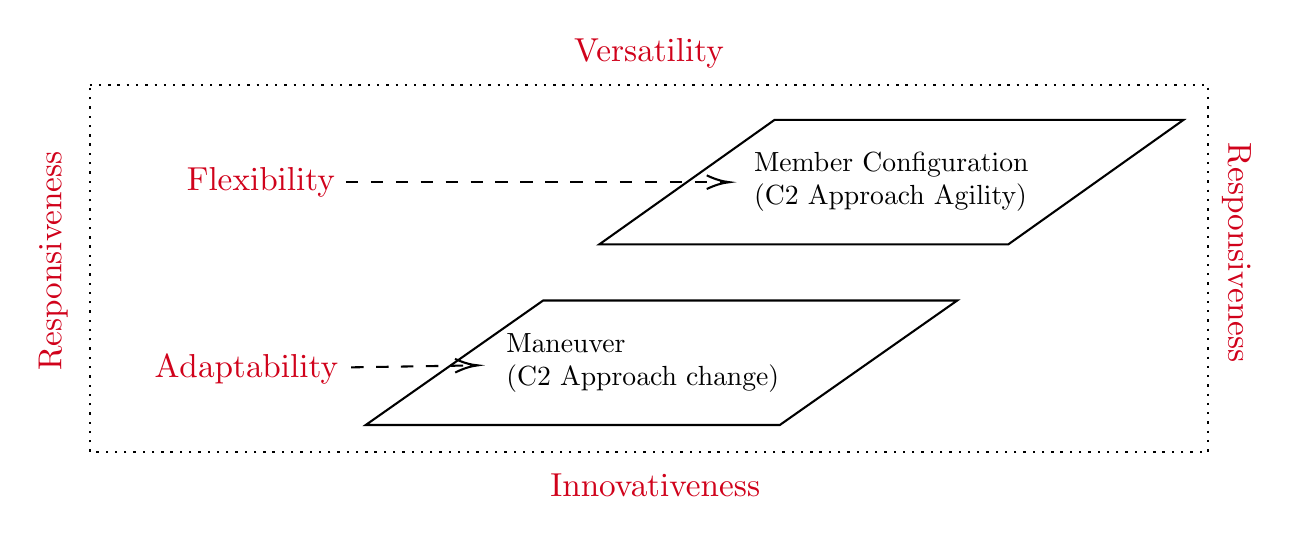
\begin{tikzpicture}[x=0.75pt,y=0.75pt,yscale=-1,xscale=1]
%uncomment if require: \path (0,300); %set diagram left start at 0, and has height of 300

%Shape: Parallelogram [id:dp7907142126701554] 
\draw   (403.45,75) -- (600.5,75) -- (516.05,135) -- (319,135) -- cycle ;
%Shape: Parallelogram [id:dp17448736771004936] 
\draw   (292,162) -- (491.5,162) -- (406,222) -- (206.5,222) -- cycle ;
%Shape: Rectangle [id:dp986244490027876] 
\draw  [dash pattern={on 0.84pt off 2.51pt}] (73.5,58) -- (612.5,58) -- (612.5,235) -- (73.5,235) -- cycle ;

% Text Node
\draw (459.75,105) node  [align=left] {Member Configuration\\(C2 Approach Agility)};
% Text Node
\draw (340,192) node  [align=left] {	Maneuver\\(C2 Approach change)};
% Text Node
\draw (343,43) node [scale=1.2,color={rgb, 255:red, 208; green, 2; blue, 27 }  ,opacity=1 ] [align=left] {Versatility};
% Text Node
\draw (346,251) node [scale=1.2,color={rgb, 255:red, 208; green, 2; blue, 27 }  ,opacity=1 ] [align=left] {Innovativeness};
% Text Node
\draw (156,105) node [scale=1.2,color={rgb, 255:red, 208; green, 2; blue, 27 }  ,opacity=1 ] [align=left] {Flexibility};
% Text Node
\draw (149,195) node [scale=1.2,color={rgb, 255:red, 208; green, 2; blue, 27 }  ,opacity=1 ] [align=left] {Adaptability};
% Text Node
\draw (626,139) node [scale=1.2,color={rgb, 255:red, 208; green, 2; blue, 27 }  ,opacity=1 ,rotate=-90] [align=left] {Responsiveness};
% Text Node
\draw (56,143) node [scale=1.2,color={rgb, 255:red, 208; green, 2; blue, 27 }  ,opacity=1 ,rotate=-270] [align=left] {Responsiveness};
% Connection
\draw  [dash pattern={on 4.5pt off 4.5pt}]  (199.5,194.21) -- (258.5,193.28) ;
\draw [shift={(260.5,193.25)}, rotate = 539.1] [color={rgb, 255:red, 0; green, 0; blue, 0 }  ][line width=0.75]    (10.93,-3.29) .. controls (6.95,-1.4) and (3.31,-0.3) .. (0,0) .. controls (3.31,0.3) and (6.95,1.4) .. (10.93,3.29)   ;

% Connection
\draw  [dash pattern={on 4.5pt off 4.5pt}]  (197,105) -- (379.75,105) ;
\draw [shift={(381.75,105)}, rotate = 180] [color={rgb, 255:red, 0; green, 0; blue, 0 }  ][line width=0.75]    (10.93,-3.29) .. controls (6.95,-1.4) and (3.31,-0.3) .. (0,0) .. controls (3.31,0.3) and (6.95,1.4) .. (10.93,3.29)   ;


\end{tikzpicture}
\caption{C2 Agility enablers linked to the analysis proposal}
\end{figure}


\section{Modelling}
\label{sec:modelling}
The members of the C2 System interacts with each other, exchanging information and awareness, and the variables evolved in these operations with all conditional rules need to be formalized. The representation chosen, called Program Graph (PG), is applied over a set of typed variables and it is represented by the following tuple:

\begin{center}
    $(Loc,Act,Effect,\lhookrightarrow,Loc_0,g_0)$
\end{center}

where,

\begin{itemize}
	\item $Loc$ is a set of location  
	\item $Act$ is a set of actions
	\item Effect is a function defined by $Act \times Eval(Var) \to Eval(Var)$
	\item $\lhookrightarrow$ is the conditional transition relation defined by $Loc \times Cond(Var) \times Act \times Loc$
	\item $Loc_0 \subseteq Loc$ is the set of initial locations
	\item $g_0 \in Cond(Var)$ is the initial condition
\end{itemize}


This representation applies conditional rules, actions and map effects over these variables, conducting the system or entity to different states. \cite{baier}. Our basic element, i.e., the DSPL, had its states modelled with this technique.

As the C2 Domain deals with dynamic context and it is under the effects of changes in the circumstances, the element representation needs to operate with variables that represents this circumstance and its dynamism. Based on the domain studies, these changes can be classified in three categories: self, environment and mission.

The pair formed by the element status ($E$) and the list of tasks allocated ($T$) represent all those changes categories. According to the mission change, the list of tasks allocated can change, adding or removing tasks from it. The sensors on board are able to obtain new conditions from the environment and its possible changes. Besides that, the element $E$ (DSPL) is represented by its feature model ($FM$) that groups all possible valid configurations that it can get during the execution. It represents the changes in the self.

Basically, the element $E$ assumes a valid configuration $c \in \llbracket FM \rrbracket$ and it has a set of tasks ($T$) allocated to be performed. The system is represented by three roles: C2 Approach Selector (C2A), Task Allocator (TA) and Executor (EX). Its execution is performed in a parallel way with data exchange through synchronous and asynchronous channels. The equation \eqref{pg01} shows the PG execution.

\begin{equation}
\label{pg01}
    PG = [C2A | TA | EX]
\end{equation}

The scenario operated by this work requires a variable sharing mechanism to guarantee an information exchange between the processes that are parts of C2 Agility.  We use a Channel System (CS) strategy to represent the system with its three roles working in a parallel way and process a communication among each other using a buffer structure, implemented as a first-in-first-out queue called channel.

Figure \ref{c2a} shows the PG that represents the C2 Approach (C2A) selection role followed by its elements. The element \textit{E} is one member with its status and configuration.

\begin{figure}[h]
\centering
\begin{center}
\end{center}
\begin{center}
\end{center}



\tikzset{every picture/.style={line width=0.75pt}} %set default line width to 0.75pt        

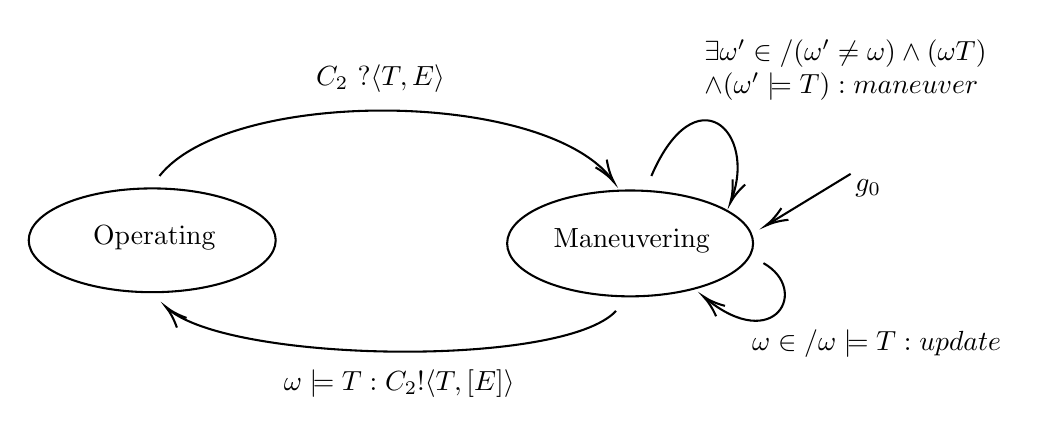
\begin{tikzpicture}[x=0.75pt,y=0.75pt,yscale=-1,xscale=1]
%uncomment if require: \path (0,215); %set diagram left start at 0, and has height of 215

%Curve Lines [id:da9480858267519683] 
\draw    (135.5,88) .. controls (169.16,45.43) and (320.43,45.98) .. (353.53,89.66) ;
\draw [shift={(354.5,91)}, rotate = 235.44] [color={rgb, 255:red, 0; green, 0; blue, 0 }  ][line width=0.75]    (10.93,-3.29) .. controls (6.95,-1.4) and (3.31,-0.3) .. (0,0) .. controls (3.31,0.3) and (6.95,1.4) .. (10.93,3.29)   ;

%Shape: Ellipse [id:dp6594609066072359] 
\draw   (72.5,119) .. controls (72.5,105.19) and (99.14,94) .. (132,94) .. controls (164.86,94) and (191.5,105.19) .. (191.5,119) .. controls (191.5,132.81) and (164.86,144) .. (132,144) .. controls (99.14,144) and (72.5,132.81) .. (72.5,119) -- cycle ;
%Shape: Ellipse [id:dp873836537729809] 
\draw   (303,120.5) .. controls (303,106.42) and (329.53,95) .. (362.25,95) .. controls (394.97,95) and (421.5,106.42) .. (421.5,120.5) .. controls (421.5,134.58) and (394.97,146) .. (362.25,146) .. controls (329.53,146) and (303,134.58) .. (303,120.5) -- cycle ;
%Curve Lines [id:da3135064064897334] 
\draw    (355.5,153) .. controls (329.89,180.58) and (170.39,178.08) .. (139.81,152.2) ;
\draw [shift={(138.5,151)}, rotate = 405] [color={rgb, 255:red, 0; green, 0; blue, 0 }  ][line width=0.75]    (10.93,-3.29) .. controls (6.95,-1.4) and (3.31,-0.3) .. (0,0) .. controls (3.31,0.3) and (6.95,1.4) .. (10.93,3.29)   ;

%Curve Lines [id:da21020703050779688] 
\draw    (372.5,88) .. controls (393.68,38.75) and (423.59,66.15) .. (411.1,99.47) ;
\draw [shift={(410.5,101)}, rotate = 292.38] [color={rgb, 255:red, 0; green, 0; blue, 0 }  ][line width=0.75]    (10.93,-3.29) .. controls (6.95,-1.4) and (3.31,-0.3) .. (0,0) .. controls (3.31,0.3) and (6.95,1.4) .. (10.93,3.29)   ;

%Curve Lines [id:da14662580418826565] 
\draw    (426.5,130) .. controls (449.16,142.81) and (432.03,174.04) .. (399.02,147.26) ;
\draw [shift={(397.5,146)}, rotate = 400.46000000000004] [color={rgb, 255:red, 0; green, 0; blue, 0 }  ][line width=0.75]    (10.93,-3.29) .. controls (6.95,-1.4) and (3.31,-0.3) .. (0,0) .. controls (3.31,0.3) and (6.95,1.4) .. (10.93,3.29)   ;

%Straight Lines [id:da37650774099478246] 
\draw    (468.5,87) -- (429.21,110.96) ;
\draw [shift={(427.5,112)}, rotate = 328.63] [color={rgb, 255:red, 0; green, 0; blue, 0 }  ][line width=0.75]    (10.93,-3.29) .. controls (6.95,-1.4) and (3.31,-0.3) .. (0,0) .. controls (3.31,0.3) and (6.95,1.4) .. (10.93,3.29)   ;


% Text Node
\draw (133,118) node  [align=left] {Operating};
% Text Node
\draw (363,119) node  [align=left] {Maneuvering};
% Text Node
\draw (242,41) node   {$C_{2} \ ?\langle T,E\rangle $};
% Text Node
\draw (251,188) node   {$\omega \models T:C_{2} !\langle T,[ E] \rangle $};
% Text Node
\draw (477,94) node   {$g_{0}$};
% Text Node
\draw (481,169) node   {$\nexists \omega \in \si{\ohm}/\omega \models T:update$};
% Text Node
\draw (466,37) node   {$ \begin{array}{l}
\exists \omega '\in \si{\ohm}/( \omega '\neq \omega ) \land ( \omega \nvDash T)\\
\land ( \omega '\models T) :maneuver
\end{array}$};


\end{tikzpicture}
\label{c2a}
\caption{C2 Approach selector PG}
\end{figure}

\begin{enumerate}
    \item $g_0=\{\omega\in\Omega,T\subseteq M\} $
    
    \item $Loc=\{Operating, Maneuvering\} $
    
    \item $Loc_0=\{Maneuvering\} $
    
    \item $Var=\{find\_maneuver(\omega,\{E\},T), f\_remove(T), \omega, T, E\} $
    
    \item $Cap(C_2)=0 $
    
    \item $\Omega=\{Edge, De-Conflicted, Coord, Conflicted, Collab \}$
    
\end{enumerate}

The effects caused by the actions are defined by

    \qquad $Effect(maneuver, \eta)= \eta[\omega:= find\_maneuver(\omega, \{E\}, T)]$
    
    \qquad $Effect(update, \eta): \eta[T:=f\_remove(T)]$
    


The $f\_remove$ function is responsible to generate a $T' \subseteq T$ such that 

\begin{center}
$ \exists \omega \in \Omega / \omega \models T' $
\end{center}

We can list the following property of the PG presented in \ref{pg01}:

\begin{center}
$ \square (\diamond Operating) $
\end{center}

Task Allocator role is represented by the PG in Figure \ref{ta} where

\begin{enumerate}

    \item $Loc=\{C2A Selecting, Idle, Updating, Allocating, Binding, Notifying \}$
    
    \item $Loc_0=\{Idle\}$
    
    \item $Var=\{alloc, f\_alloc, T, E, t\} $
    
    \item $Cap(C_2)=0 $
    
    \item $Cap(C_1)>0 $
    
    \item $Cap(m_k)>0 $
    
    \item $alloc=\{\langle k,T \rangle\}  $
\end{enumerate}

$k$ variable represents the index of the element $E$ in the set of all agents ($\{E\}$) and it is in the interval $[1..|\{E\}|]$ . T is a set of tasks $t$. The effects of the actions are defined by:

\qquad $Effect(allocate, \eta)= \eta[alloc:= f\_alloc(T, \{E\})]$
    
\qquad $Effect(bind, \eta): \eta[\langle k,T \rangle:=head(alloc); alloc:=tail(alloc)]$

\begin{figure}[h]
\centering
\begin{center}
\end{center}
\begin{center}
\end{center}



\tikzset{every picture/.style={line width=0.75pt}} %set default line width to 0.75pt        

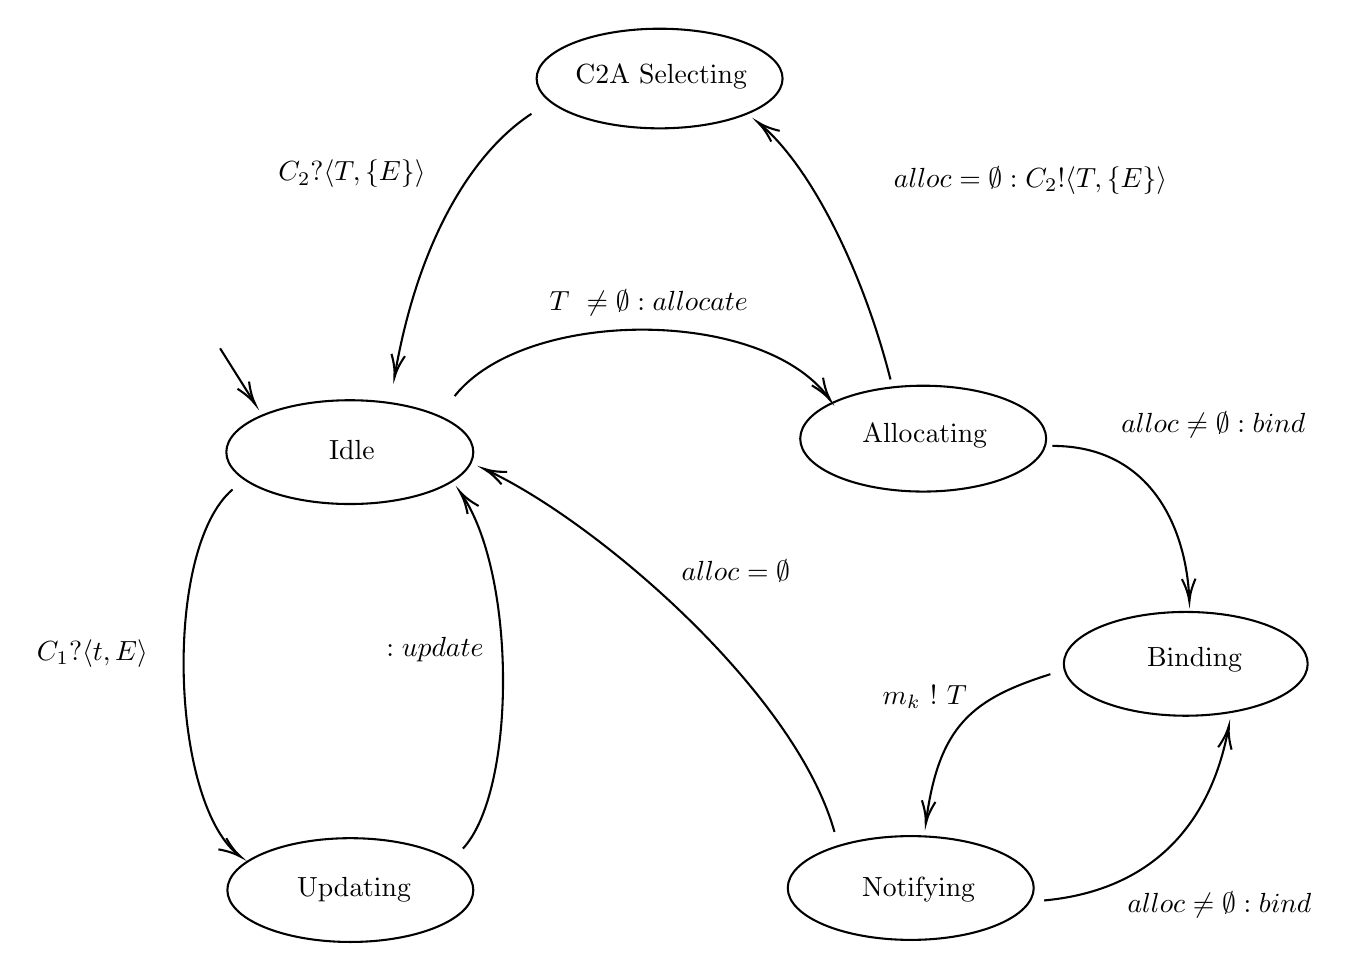
\begin{tikzpicture}[x=0.75pt,y=0.75pt,yscale=-1,xscale=1]
%uncomment if require: \path (0,455); %set diagram left start at 0, and has height of 455

%Curve Lines [id:da9480858267519683] 
\draw    (230.5,181) .. controls (264.16,138.43) and (378.19,138) .. (410.54,181.66) ;
\draw [shift={(411.5,183)}, rotate = 235.44] [color={rgb, 255:red, 0; green, 0; blue, 0 }  ][line width=0.75]    (10.93,-3.29) .. controls (6.95,-1.4) and (3.31,-0.3) .. (0,0) .. controls (3.31,0.3) and (6.95,1.4) .. (10.93,3.29)   ;

%Shape: Ellipse [id:dp6594609066072359] 
\draw   (120.5,208) .. controls (120.5,194.19) and (147.14,183) .. (180,183) .. controls (212.86,183) and (239.5,194.19) .. (239.5,208) .. controls (239.5,221.81) and (212.86,233) .. (180,233) .. controls (147.14,233) and (120.5,221.81) .. (120.5,208) -- cycle ;
%Shape: Ellipse [id:dp873836537729809] 
\draw   (397,201.5) .. controls (397,187.42) and (423.53,176) .. (456.25,176) .. controls (488.97,176) and (515.5,187.42) .. (515.5,201.5) .. controls (515.5,215.58) and (488.97,227) .. (456.25,227) .. controls (423.53,227) and (397,215.58) .. (397,201.5) -- cycle ;
%Curve Lines [id:da14662580418826565] 
\draw    (514.5,424) .. controls (567.96,419.05) and (594.96,385.68) .. (603.25,341.35) ;
\draw [shift={(603.5,340)}, rotate = 460.08] [color={rgb, 255:red, 0; green, 0; blue, 0 }  ][line width=0.75]    (10.93,-3.29) .. controls (6.95,-1.4) and (3.31,-0.3) .. (0,0) .. controls (3.31,0.3) and (6.95,1.4) .. (10.93,3.29)   ;

%Straight Lines [id:da37650774099478246] 
\draw    (117.5,158) -- (133.43,183.31) ;
\draw [shift={(134.5,185)}, rotate = 237.8] [color={rgb, 255:red, 0; green, 0; blue, 0 }  ][line width=0.75]    (10.93,-3.29) .. controls (6.95,-1.4) and (3.31,-0.3) .. (0,0) .. controls (3.31,0.3) and (6.95,1.4) .. (10.93,3.29)   ;

%Shape: Ellipse [id:dp8139093405894636] 
\draw   (121,419) .. controls (121,405.19) and (147.53,394) .. (180.25,394) .. controls (212.97,394) and (239.5,405.19) .. (239.5,419) .. controls (239.5,432.81) and (212.97,444) .. (180.25,444) .. controls (147.53,444) and (121,432.81) .. (121,419) -- cycle ;
%Shape: Ellipse [id:dp08678607998247811] 
\draw   (391,418) .. controls (391,404.19) and (417.53,393) .. (450.25,393) .. controls (482.97,393) and (509.5,404.19) .. (509.5,418) .. controls (509.5,431.81) and (482.97,443) .. (450.25,443) .. controls (417.53,443) and (391,431.81) .. (391,418) -- cycle ;
%Shape: Ellipse [id:dp07482494496489733] 
\draw   (270,28) .. controls (270,14.75) and (296.53,4) .. (329.25,4) .. controls (361.97,4) and (388.5,14.75) .. (388.5,28) .. controls (388.5,41.25) and (361.97,52) .. (329.25,52) .. controls (296.53,52) and (270,41.25) .. (270,28) -- cycle ;
%Curve Lines [id:da6759956440889884] 
\draw    (123.5,226) .. controls (90.01,254.57) and (93.39,375.3) .. (125.99,401.85) ;
\draw [shift={(127.5,403)}, rotate = 215.22] [color={rgb, 255:red, 0; green, 0; blue, 0 }  ][line width=0.75]    (10.93,-3.29) .. controls (6.95,-1.4) and (3.31,-0.3) .. (0,0) .. controls (3.31,0.3) and (6.95,1.4) .. (10.93,3.29)   ;

%Curve Lines [id:da9572857730465772] 
\draw    (234.22,228.76) .. controls (260.49,268.16) and (260.11,371.42) .. (234.5,399) ;

\draw [shift={(233,227)}, rotate = 54.11] [color={rgb, 255:red, 0; green, 0; blue, 0 }  ][line width=0.75]    (10.93,-3.29) .. controls (6.95,-1.4) and (3.31,-0.3) .. (0,0) .. controls (3.31,0.3) and (6.95,1.4) .. (10.93,3.29)   ;
%Curve Lines [id:da9385545433271328] 
\draw    (517.5,315) .. controls (479.88,326.88) and (463.82,339.74) .. (457.68,385.6) ;
\draw [shift={(457.5,387)}, rotate = 277.28] [color={rgb, 255:red, 0; green, 0; blue, 0 }  ][line width=0.75]    (10.93,-3.29) .. controls (6.95,-1.4) and (3.31,-0.3) .. (0,0) .. controls (3.31,0.3) and (6.95,1.4) .. (10.93,3.29)   ;

%Curve Lines [id:da13526468384837043] 
\draw    (440.5,173) .. controls (426.78,119.1) and (401.54,70) .. (377.94,50.18) ;
\draw [shift={(376.5,49)}, rotate = 398.37] [color={rgb, 255:red, 0; green, 0; blue, 0 }  ][line width=0.75]    (10.93,-3.29) .. controls (6.95,-1.4) and (3.31,-0.3) .. (0,0) .. controls (3.31,0.3) and (6.95,1.4) .. (10.93,3.29)   ;

%Curve Lines [id:da7876400787103589] 
\draw    (267.5,45) .. controls (238.79,63.81) and (213.02,106.14) .. (201.83,170.06) ;
\draw [shift={(201.5,172)}, rotate = 279.61] [color={rgb, 255:red, 0; green, 0; blue, 0 }  ][line width=0.75]    (10.93,-3.29) .. controls (6.95,-1.4) and (3.31,-0.3) .. (0,0) .. controls (3.31,0.3) and (6.95,1.4) .. (10.93,3.29)   ;

%Shape: Ellipse [id:dp538933115831977] 
\draw   (524,310) .. controls (524,296.19) and (550.3,285) .. (582.75,285) .. controls (615.2,285) and (641.5,296.19) .. (641.5,310) .. controls (641.5,323.81) and (615.2,335) .. (582.75,335) .. controls (550.3,335) and (524,323.81) .. (524,310) -- cycle ;
%Curve Lines [id:da663291454681702] 
\draw    (518.5,205) .. controls (566.52,205) and (582.85,245.34) .. (584.42,278.01) ;
\draw [shift={(584.5,280)}, rotate = 268.26] [color={rgb, 255:red, 0; green, 0; blue, 0 }  ][line width=0.75]    (10.93,-3.29) .. controls (6.95,-1.4) and (3.31,-0.3) .. (0,0) .. controls (3.31,0.3) and (6.95,1.4) .. (10.93,3.29)   ;

%Curve Lines [id:da17641910717404863] 
\draw    (413.5,391) .. controls (394.69,323.68) and (299.43,241.66) .. (246.1,216.74) ;
\draw [shift={(244.5,216)}, rotate = 384.36] [color={rgb, 255:red, 0; green, 0; blue, 0 }  ][line width=0.75]    (10.93,-3.29) .. controls (6.95,-1.4) and (3.31,-0.3) .. (0,0) .. controls (3.31,0.3) and (6.95,1.4) .. (10.93,3.29)   ;


% Text Node
\draw (181,207) node  [align=left] {Idle};
% Text Node
\draw (457,200) node  [align=left] {Allocating};
% Text Node
\draw (324,136) node   {$T\ \neq \emptyset :allocate$};
% Text Node
\draw (182,419) node  [align=left] {Updating};
% Text Node
\draw (454,419) node  [align=left] {Notifying};
% Text Node
\draw (330,27) node  [align=left] {C2A Selecting};
% Text Node
\draw (56,305) node   {$C_{1} ?\langle t,E\rangle $};
% Text Node
\draw (221,303) node   {$:update$};
% Text Node
\draw (508,77) node   {$alloc=\emptyset :C_{2} !\langle T,\{E\} \rangle $};
% Text Node
\draw (181,74) node   {$C_{2} ?\langle T,\{E\} \rangle $};
% Text Node
\draw (587,308) node  [align=left] {Binding};
% Text Node
\draw (599,426) node   {$alloc\neq \emptyset :bind$};
% Text Node
\draw (457,326) node   {$m_{k\ } !\ T$};
% Text Node
\draw (596,195) node   {$alloc\neq \emptyset :bind$};
% Text Node
\draw (366,265) node   {$alloc=\emptyset $};


\end{tikzpicture}
\label{ta}
\caption{Task Allocator PG}
\end{figure}

Property: 

\begin{center}
$ \square (\diamond Idle) $
\end{center}

The task allocator will be called by the task executor, that is defined by the program graph in Figure \ref{executor}.

\begin{figure}[h]
\centering
\begin{center}
\end{center}
\begin{center}
\end{center}
\begin{center}
\end{center}



\tikzset{every picture/.style={line width=0.75pt}} %set default line width to 0.75pt        

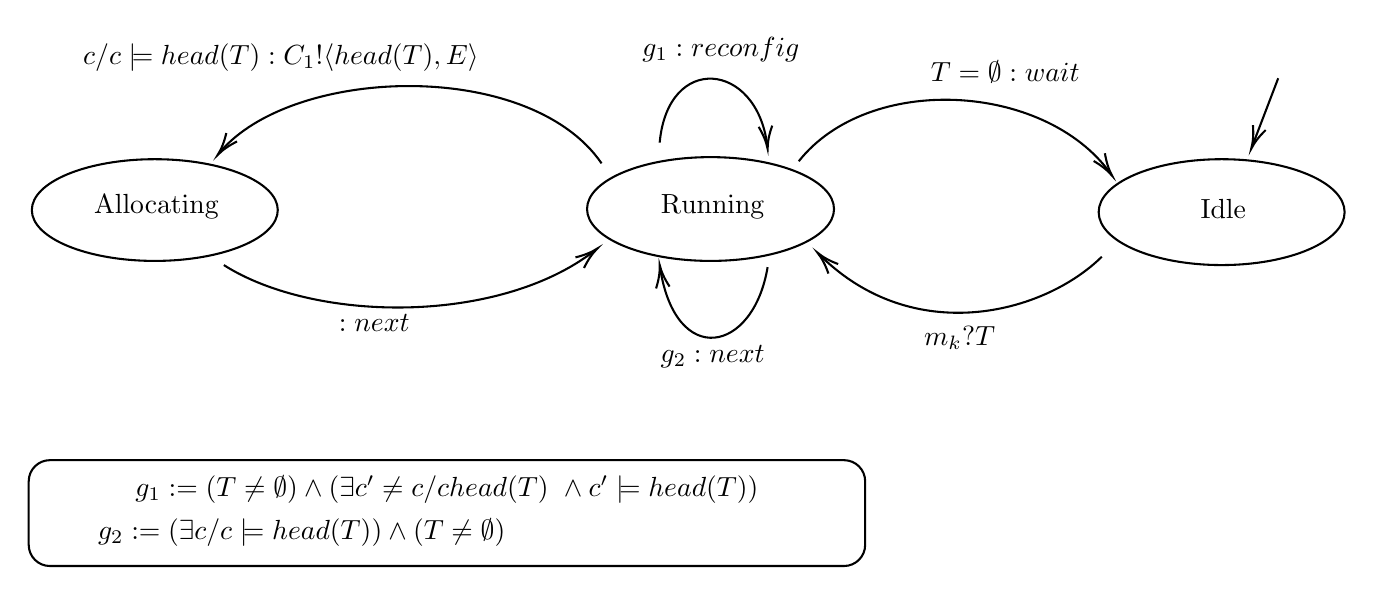
\begin{tikzpicture}[x=0.75pt,y=0.75pt,yscale=-1,xscale=1]
%uncomment if require: \path (0,306); %set diagram left start at 0, and has height of 306

%Curve Lines [id:da9480858267519683] 
\draw    (379.5,108) .. controls (413.16,65.43) and (497.79,69.9) .. (529.55,113.66) ;
\draw [shift={(530.5,115)}, rotate = 235.44] [color={rgb, 255:red, 0; green, 0; blue, 0 }  ][line width=0.75]    (10.93,-3.29) .. controls (6.95,-1.4) and (3.31,-0.3) .. (0,0) .. controls (3.31,0.3) and (6.95,1.4) .. (10.93,3.29)   ;

%Shape: Ellipse [id:dp6594609066072359] 
\draw   (277.5,131) .. controls (277.5,117.19) and (304.14,106) .. (337,106) .. controls (369.86,106) and (396.5,117.19) .. (396.5,131) .. controls (396.5,144.81) and (369.86,156) .. (337,156) .. controls (304.14,156) and (277.5,144.81) .. (277.5,131) -- cycle ;
%Shape: Ellipse [id:dp873836537729809] 
\draw   (524,132.5) .. controls (524,118.42) and (550.53,107) .. (583.25,107) .. controls (615.97,107) and (642.5,118.42) .. (642.5,132.5) .. controls (642.5,146.58) and (615.97,158) .. (583.25,158) .. controls (550.53,158) and (524,146.58) .. (524,132.5) -- cycle ;
%Curve Lines [id:da3135064064897334] 
\draw    (364.5,159) .. controls (357.57,200.58) and (320.26,207.86) .. (312.72,159.48) ;
\draw [shift={(312.5,158)}, rotate = 442.03] [color={rgb, 255:red, 0; green, 0; blue, 0 }  ][line width=0.75]    (10.93,-3.29) .. controls (6.95,-1.4) and (3.31,-0.3) .. (0,0) .. controls (3.31,0.3) and (6.95,1.4) .. (10.93,3.29)   ;

%Curve Lines [id:da21020703050779688] 
\draw    (312.5,99) .. controls (316.44,55.66) and (359.19,59.86) .. (364.29,100.14) ;
\draw [shift={(364.5,102)}, rotate = 264.56] [color={rgb, 255:red, 0; green, 0; blue, 0 }  ][line width=0.75]    (10.93,-3.29) .. controls (6.95,-1.4) and (3.31,-0.3) .. (0,0) .. controls (3.31,0.3) and (6.95,1.4) .. (10.93,3.29)   ;

%Straight Lines [id:da37650774099478246] 
\draw    (610.5,68) -- (598.21,100.13) ;
\draw [shift={(597.5,102)}, rotate = 290.92] [color={rgb, 255:red, 0; green, 0; blue, 0 }  ][line width=0.75]    (10.93,-3.29) .. controls (6.95,-1.4) and (3.31,-0.3) .. (0,0) .. controls (3.31,0.3) and (6.95,1.4) .. (10.93,3.29)   ;

%Shape: Ellipse [id:dp02234558999259495] 
\draw   (10,131.5) .. controls (10,117.97) and (36.53,107) .. (69.25,107) .. controls (101.97,107) and (128.5,117.97) .. (128.5,131.5) .. controls (128.5,145.03) and (101.97,156) .. (69.25,156) .. controls (36.53,156) and (10,145.03) .. (10,131.5) -- cycle ;
%Curve Lines [id:da2517277021570281] 
\draw    (284.5,109) .. controls (249.85,58.51) and (135.81,61.93) .. (100.54,103.72) ;
\draw [shift={(99.5,105)}, rotate = 308.33000000000004] [color={rgb, 255:red, 0; green, 0; blue, 0 }  ][line width=0.75]    (10.93,-3.29) .. controls (6.95,-1.4) and (3.31,-0.3) .. (0,0) .. controls (3.31,0.3) and (6.95,1.4) .. (10.93,3.29)   ;

%Curve Lines [id:da851947022127026] 
\draw    (102.5,158) .. controls (146.06,185.72) and (234.7,186.98) .. (281.11,151.1) ;
\draw [shift={(282.5,150)}, rotate = 501.19] [color={rgb, 255:red, 0; green, 0; blue, 0 }  ][line width=0.75]    (10.93,-3.29) .. controls (6.95,-1.4) and (3.31,-0.3) .. (0,0) .. controls (3.31,0.3) and (6.95,1.4) .. (10.93,3.29)   ;

%Curve Lines [id:da05773774536505705] 
\draw    (525.5,154) .. controls (497.29,181.72) and (434.77,197.68) .. (389.86,153.36) ;
\draw [shift={(388.5,152)}, rotate = 405.63] [color={rgb, 255:red, 0; green, 0; blue, 0 }  ][line width=0.75]    (10.93,-3.29) .. controls (6.95,-1.4) and (3.31,-0.3) .. (0,0) .. controls (3.31,0.3) and (6.95,1.4) .. (10.93,3.29)   ;

%Rounded Rect [id:dp5913972444482631] 
\draw   (8.5,262.2) .. controls (8.5,256.57) and (13.07,252) .. (18.7,252) -- (401.3,252) .. controls (406.93,252) and (411.5,256.57) .. (411.5,262.2) -- (411.5,292.8) .. controls (411.5,298.43) and (406.93,303) .. (401.3,303) -- (18.7,303) .. controls (13.07,303) and (8.5,298.43) .. (8.5,292.8) -- cycle ;

% Text Node
\draw (338,130) node  [align=left] {Running};
% Text Node
\draw (584,131) node  [align=left] {Idle};
% Text Node
\draw (479,65) node   {$T=\emptyset :wait$};
% Text Node
\draw (130,58) node   {$\nexists c/c\models head( T) :C_{1} !\langle head( T) ,E\rangle $};
% Text Node
\draw (457,193) node   {$m_{k} ?T$};
% Text Node
\draw (70,130) node  [align=left] {Allocating};
% Text Node
\draw (175,186) node   {$:next$};
% Text Node
\draw (210,266) node   {$g_{1} :=( T\neq \emptyset ) \land ( \exists c'\neq c/c\nvDash head( T) \ \land c'\models head( T))$};
% Text Node
\draw (342,54) node   {$g_{1} :reconfig$};
% Text Node
\draw (338,202) node   {$g_{2} :next$};
% Text Node
\draw (140,287) node   {$g_{2} :=( \exists c/c\models head( T)) \land ( T\neq \emptyset )$};


\end{tikzpicture}
\label{executor}
\caption{Task Executor PG}
\end{figure}

Its elements is listed below:

\begin{enumerate}

    \item $Loc=\{Running, Idle, Allocating \}$
    
    \item $Loc_0=\{Idle\}$
    
    \item $Var=\{T, E, c\} $
    
    \item $Cap(C_1)>0 $
    
    \item $Cap(m_k)>0 $
    
\end{enumerate}

where $k$ indicates the index of the executor in analysis.

The effects of the actions are defined by

\qquad $Effect(reconfig, \eta)= \eta[c:=c']$
    
\qquad $Effect(next, \eta): \eta[T:=tail(T)]$

\qquad $Effect(wait, \eta): \eta$

For the task executor, the following properties can be identified:

\qquad $\square \diamond (Idle)$

\qquad $\diamond Running$

\begin{figure}[h]
\centering
\input{tiks/states.tex}
\caption{Set of member's valid states}
\end{figure}


\section{Equations and Formulas}

The context is formed by the mission, the environment and the self (members themselves). Any of these elements can suffer modifications and the possible system situations are the following:
\begin{enumerate}
    \item All members that form the teams are performing the tasks with no special adjustments in runtime (even not being all mission defined by a set of tasks). This is the normal situation.
    \item The context changes cause a reconfiguration in one or more member such as a DSPL structure. This represents C2 Approach Agility that indicates the capability of the system to adapt itself with no C2 Approach changes. In this case, with information about the tasks to be performed, each member will reconfigure itself to try to stabilize the system, allocating all possible tasks available.
    \item In case of C2 Approach Agility does not work, it is necessary to try a C2 Approach change to deal with a new context. The members will be organized according to a C2 Approach selected and analyze if the tasks can be performed. The new coordination will impact the task allocation procedure. The capability of getting a C2 Approach to deal with context changes defines the C2 Meneuver Agility level.
    \item No members configuration and C2 Approach are suitable to perform the tasks. Complete C2 System Failure.
\end{enumerate}

Many environment changes, e.g., risk level increase or security requirements are treated as a factor that needs to be observed by someone and triggered manually in the system.

Following is shown the logic formulas that represents the situations listed above. The mission to be accomplished is formed by a set of tasks $T=\{t_1, t_2, t_3,...\}$. The set of members is $M = \{m_1, m_2, m_3,... \}$, and each member $m_k$ has a set of possible and valid configurations $C_k = \{c_{1k}, c_{2k}, c_{3k}, ... \}$. A member $m_k$ can have a set $t_k \subseteq T$ of tasks allocated to it, and the empty set indicates no task allocated or tasks finished.

There is no collaborative work, i.e., for two different members $m_i$ and $m_j$, with $t_i, t_j \subseteq T$\, it is valid that $t_i \cap t_j = \emptyset$.

We define a team as a set $\tau$ of members such as $\tau \subseteq M$. All possible C2 Approaches (Conflicted, De-Conflicted, Coordinated, Collaborative and Edge) form the set $\Omega$. A team always has a C2 Approach $\omega \in \Omega$ applied that defines its coordination and organization. 

The Equation \eqref{eq1} shows the case 1 where the members and/or teams are executing the tasks allocated normally with no issues and operating on a C2 Approach $\omega$.

\begin{equation}
\label{eq1}
 P_1 = \forall m \in M, \exists c \in C_m ( \square (\exists t_m \subseteq T | (c, \omega) \models t_m ) \land \diamond (T = \emptyset )) 
\end{equation}

The case defined by item 2 performs a reconfiguration based on the list of tasks to be allocated. This allocation looks for maximize any quality level, e.g., sensors and tasks compatibility or time to execution. This case satisfies at least one of \eqref{eq2} and \eqref{eq3}. 

Changes in the mission, generating another set of tasks $T'$ requires a verification if the current member configuration satisfies the requirements. This situation is attended by Eq. \eqref{eq2}. When the changes affect one or more members, a reconfiguration can be necessary to reach a new configuration $c'$ and it is represented by Eq. \eqref{eq3}. The reconfiguration will occurs as a DSPL having the tasks available to define which configuration is suitable to perform those tasks, if feasible. In case of unsuccessful, they can give up the task, but always keeping the C2 Approach $\omega$.

Environment modifications is not in the scope of this study based on its complexity. These dynamic aspects will be treated as self modifications, due to the correlation among environment changes and self modification to deal with stimulus around itself.

%\begin{equation}
%\label{eq2}
% P_2 = ((\forall m \in M_f, \forall t' \subseteq T', \exists c' \in C_m %((c',\omega) \models t')) \land (T' \ne \emptyset) ) 
%\end{equation}


\begin{equation}
\label{eq2}
 P_2 = (\forall m \in M (\diamond \exists T' \ne T (\exists t'_m \subseteq T', \exists c \in C_m | (c, \omega) \models t'_m))) \land (T' \ne \emptyset)  
\end{equation}

\begin{equation}
\label{eq3}
 P_3 = (\forall m \in M (\diamond \exists c' \in C_m ( \exists t \subseteq T | (c',\omega) \models t))) \land (T \ne \emptyset)  
\end{equation}

%where $M_f \subseteq M$ is the set of members that had any issue, and $T'\subseteq T$ represents a possible mission modification.

Item 3 defines the situation that C2 Approach agility was not enough to deal with the context and a C2 Approach change is required. This case represents the C2 Maneuver agility, i.e., the agility to change among different C2 Approaches. The Eq. \eqref{eq4} shows this situation. 

\begin{equation}
\label{eq4}
 P_4 = \exists \omega' \in \Omega | P_1[\omega / \omega']
\end{equation}

From this state, all formulas operate with a variable replacement where $[\omega / \omega']$ .

Equation \eqref{eq5} represents the item 4 where the tasks were accomplished and/or the system is not able to execute the remaining tasks.

\begin{equation}
\label{eq5}
 P_5 = \diamond \square ((T = \emptyset) \lor (\neg (P_2 \lor P_3)))
\end{equation}

In all cases, we are considering the task allocation procedure as an inner action that runs together with the member reconfiguration, giving information to define right feature selection, and aiming: 1) to optimize results; 2) keep the system running; and 3) to complement the C2 Approach and member configuration changes. 


\section{State Machine}%

Based on the logical propositions presented before, a state-chart was created to represent possible system states and its transitions. When a proposition $P_n$ is satisfied, an action is executed to make a transition and adjust the system configuration.

\figura[!h]{model01}{State machine representing the system}{model01}{width=1\textwidth}%

The actions used are listed bellow:

\begin{itemize}
    \item \textbf{reconf} - makes the elements reconfiguration, as a DSPL, activating and deactivating features according to the list of tasks available, making simultaneous reallocation if it is necessary.
    \item \textbf{maneuver} - executes a C2 Approach change. It can be followed by elements reconfiguration according this new organization structure.
    \item \textbf{run} - it is the normal execution, with no kind of reconfiguration required.
    \item \textbf{finish} - it confirms the mission accomplishment or no more resources available to be allocated to tasks execution.
\end{itemize}







\subsection{Simulation environment}
We chose NetLogo\footnote{Found at http://ccl.northwestern.edu/netlogo/}, a multi-agent programmable modeling environment that permits to simulate scenarios where there are agents interacting and executing tasks under environment effects. With this tool, it is possible to analyze the agent's reactions and measure results.

\textit{Abar et al.} in \cite{ABAR201713} analyzed a large group of agent-based tools in many aspects that impact on their use, as simplicity and strength to model. Although NetLogo uses a specific language with a particular syntax, it is considered a tool with low complexity and requires medium strength to be used as a modeling tool. Furthermore, there are many extensions that can be used to include resources and to  integrate with other technologies to exchange data and results.

This tool permits to generate simulations in 2D and 3D, and it is compiled by any Java Virtual Machine (5.0 or above). Active objects with simple goals can be implemented as mobile agents and they can be showed in a dynamic way.



\subsection{Transition System}

To represent the transition system(TS) we are using Labeled Kripke Structures presented by \textit{Chaki et al.} in \cite{ltl02}. The State/Event Linear Temporal Logic (SE-LTL) extends LTL to represent temporal properties over states and actions \cite{ltl01}.

\subsection{CSP}
Constraint Satisfaction Problem: the set of values in domain that satisfies constraints defines the CSP model. A model becomes valid the result satisfying all constraints.






\subsection{Threats to Validity}
\label{sec:threats}
%Threats to validity
% scenario more dynamic
% other variables change

Basically, the methodology applied in this study was action research to explore weaknesses and not answered questions related to C2 application and its challenges. The SPL approach applied to prospect the solution proposed required some simplification in the original problem. Thus, for this process, the following threats to validity and corresponding mitigation strategies are presented in the following: 

\begin{itemize}
   \item \textbf{Conclusion validity}: 
   
   \item \textbf{Internal validity}: 
   
   \item \textbf{Construct validity}: To assure that the network structures chosen were suitable to simplify NEC approach applied to the five maturity levels in C2 Approach Space, all connectivity characteristics of each C2 approach were analyzed and compared with each network topology used as approximation. Additionally, mixed structures with complex nodes connections were ignored to becomes the solution feasible.
   
   
   \item \textbf{External validity}: This work considers a dynamic scenario to analyze problem and solution. This dynamism involves changes in the context, i.e., changes in the environment, in the element itself, and in the mission. However, our scope did not consider the environment in a broader sense. Since the complexity related to this dimension, we are working only on aspects that can be perceived by the sensors, e.g., weather changes that a humidity sensor was capable to perceive.
\end{itemize}

\subsection{Solution Proposed}
\textit{Brun et al.}\cite{SAS02} applies the definition of orthogonality in self-adaptive systems to represent independent dimensions where any modification in one of them do not cause impact on the others. They are completely independent and can be adjusted according to the requirements. In our proposed model, the two dimensions presented, as a DSPL set and a C2 Approach, are \textit{quasi-orthogonal}. In this work, we are using this term to express a partial dependence among these two dimensions. It means that changes in any of them may cause reactions in the other, but this effect is not mandatory.
